\documentclass[../OAE-SPEC-MAIN.tex]{subfiles}

\title{Bits and Bytes}

\begin{document}

\chapter{Bits and Bytes}\label{sec:bits-and-bytes}


\section{64-Byte Record}
\begin{marginfigure}[+20mm]
  \includegraphics[width=\linewidth]{./figures/64-Byte-record.pdf}
  \caption{64-Byte Record. $8\times8$ byte slices, pre-emptible by responders} %Minimum record size is 64 Bytes; comprised of 8Bytes $\times$ 8 Slices, pre-emptable by the receiver}
\end{marginfigure}


%64-Byte-Record\footnote{Frames are variable Length in ATM -- return to original Manchester encoding where \texttt{record} is fixed size [ref] }

\AE thernet operates exclusively on fixed-sized records so every transmission has bounded entropy, and pipelines can be made in the hardware with latency guarantees. Most SerDes on the market are designed to operate on 8-byte (64-bit) atomic slices, which align naturally with fixed size encoding schemes like 64b/66b and enable efficient, low-entropy, and latency-predictable data movement through hardware pipelines.

8-bytes is the atomic unit of transmission in \AE thernet, but the fundamental record size is 64 bytes, representing the maximum uninterrupted knowledge transfer permitted by a \LINK. Each frame is structured into \emph{slots} that correspond to exponentially increasing levels of entropy, at the expense of temporal intimacy.



%\begin{enumerate}
%\item The protocol prioritizes information reliability and bandwidth allocation on a Neighbor-to-Neighbor (N2N), instead of an End-to-End (E2E) principle in conventional networks.
%\item Each pair of neighbor nodes is connected \emph{directly} to its neighbor and does not go through any other device or entity.  Advantages include:
%	\begin{itemize}
%	\item Security - Connections between nodes is private and near impossible to eavesdrop on without both parties being able to detect that.
%	\item Confinement - 
%	\item Temporal intimacy -- events on one side can be precisely correlated with events on the other side
%	\end{itemize}
%\item Processing of the packets is  organized in order to process information from the inside out
%	\begin{itemize}
%	\item LINK (Fast ULL computations in the Link itself. E.g. for ML/AI linear algebra operators)
%	\item CELL (the unit of network presence, whether or not it connects via PCIe bus to a host processor
%	\item TILE (Graph computations such as consensus (Paxos/Raft), including atomic cluster management
%	\item Local Topology Awareness beyond the 1-hop (3 x 3) tile.
%	\item	Remote Topology awareness of secure enclave boundaries and gateways to the IP world
%	\end{itemize}
%\end{enumerate}

\subsection{Slot Boundaries}

\begin{marginfigure}[+40mm]
   \hspace{-18pt}    \includegraphics[width=1.12\linewidth]{./figures/slice-arrival.pdf}
  \caption{Slice Arrival order (Temporal  Intimacy Depth)}
\end{marginfigure}

In \AE thernet, each slot boundary contributes to the progressive construction of meaning. Rather than dividing slots into fixed roles (e.g., header vs payload), each slice refines the shared semantic context between sender and receiver. This unfolding process is tracked through a series of Sub-ACKs (SACKs), signaling progressively deeper certainty at four boundaries (1, 2, 4, and 8 slices). These boundaries correspond to conceptual layers of comprehension:

\begin{description}
  \item [Slice 1:] \textbf{Arrival of Context} — Establishes the physical link is live. The receiver confirms deserialization and framing; the message has landed.

  \item [Slice 2:] \textbf{Recognition of Form} — Basic headers or structure emerge. Receiver begins to interpret role and framing, setting state machines into motion.

  \item [Slices 3–4:] \textbf{Activation of Semantics} — The receiver has seen enough to begin logical interpretation: which class of message is it? What resources must it allocate?

  \item [Slices 5–8:] \textbf{Consolidation of Understanding} — With full delivery, the entire 64-byte message is interpreted as a coherent unit. At this point, delivery to the host or downstream actor becomes safe and lossless.

\end{description}

Every slice carries data, but also a layer of \textbf{epistemic weight}. The meaning of the message doesn't come from a single part, but from the \textbf{cumulative structure of all slices}, layered like a wavefunction collapsing toward certainty.



\subsection{Pre-Emption}

In \AE thernet, it is the responsibility of the receiver to jam the sender and borrow the sender's token to transfer a frame the receiver wants to send. Due to physical limitations, the first few slices will arrive at the receiver before the jam signal contained in the first slice acknowledgement will override the frame's ownership to the receiver until the other side jams for ownership.

This allows one side of the link to jam the other side and utilize the full interaction capacity of the link for its frames. Pre-emption is decided on the first slice acknowledgement, until the other side has something it needs to send, and jams for ownership of one or both snakes. 

There is no jam hierarchy or recursive jamming, frame ownership is a state owned entirely by the \LINK and the \LINK state machines determine when a frame is jammed for ownership. The jammed frame is immediately removed from the sender's queue, and ownership of the jammed frame is returned to the controller for possible re-routing or to jam the frame in at some backoff.

To ensure fair use of frames for maximum throughput, each link communicates status frames with the other side for leaning throughput in one direction or the other.






%\subsection{Protocol hierarchy:  Four levels of Reversibility:}

%\begin{itemize}
%\item Context Slice Reversibility 
%\item Shannon Information (Operand Zone A in Serdes)
%\item Spekkens Knowledge (Operand Zone B  FPGAs, 2-3 clock cycles in)
%\item Metcalfe Semantics (Operand Zone C in FPGA, 5-8 clock cycles in)
%\end{itemize}


%\subsection{Extended Addressing Modes for Legacy Compatibility}

%To guarantee that no information is lost %\footnote[][-20mm]{All distributed systems need transactions. Even applications that run on a single (multicore) machine need them.  If it runs in the cloud, it needs a transactional infrastructure underneath.}% to provide tenant provisioning \& isolation.}, 
%the slots must be fixed size.  PCIe and CXL attempt to transfer 64 bytes minimum.  This makes the latency (occupation time on the wire) too long for ULL applications. Instead, we propose a minimum of the first slice (Protocol  -- Context).  Optional second slice  (Reliability/Recoverability). The rest is payload for local Ultra-Low-Latency (ULL) Transactions.

%\begin{description}
%\item [Mode 1]- N2N Neighbor Self-Addressing
%\item [Mode 2]- Ethernet MAC Addressing
%\item [Mode 3]- 32-Bit IP Addressing
%\item [Mode 4]- 128-Bit IP Addressing (Container virtual addresses?)
%\item [Mode 5]- 10-Bit Cluster Addressing 12-bit VLAN Addressing.
%\item [Modes 6..8]- Reserved
%\item [Mode 7]- Reserved
%\item [Mode 8]- Reserved
%\end{description}


\section{Flow Transactions}
%\marginnote{See \href{https://en.wikipedia.org/wiki/Ethernet_frame}{Ethernet Frame on Wikipedia}} 

\begin{marginfigure}[-55mm]
  \includegraphics[width=\linewidth]{./figures/1-slice.pdf}
  \caption{1  Slice Flow Subtransaction}
\end{marginfigure}

\begin{marginfigure}[-20mm]
    \includegraphics[width=\linewidth]{./figures/2-slice-operator.pdf}
  \caption{2 slice  Flow SubTransaction}% with 12B payload (operand)}
\end{marginfigure}

\begin{marginfigure}
      \includegraphics[width=\linewidth]{./figures/4-slice-operator.pdf}
  \caption{4 4 slice Flow SubTransaction with 28B payload (operand) \vspace{15pt}} % TODO Extraneous vspace. Need to eliminate
\end{marginfigure}

\begin{marginfigure}
        \includegraphics[width=\linewidth]{./figures/8-slice-operator.pdf}
  \caption{1 $\times$ 8 slice Flow  Transaction with 60B payload}
\end{marginfigure}

ULL protocol designers play around with 32 bits as the minimum unit of transactional transfer, but experiments demonstrate the difficulty of making this consistently reliable i; the general consensus is that modern SerDes' work best with $\ge 64$ bit (8 Byte) slices/flits.
%Google Aquila, uses 16 byte flits.
Ethernet  has a minimum frame size of 64 bytes  (although only 42 bytes were available for the payload).

We therefore choose a \emph{fixed} 64 Byte frame for the Shannon Slots, but make them \emph{pre-emptable} so that even the minimum size frame does not need to occupy space on the wire, increase latency, or FPGA processing steps, when the receiver has something more important it wishes to send (e.g. local status messages sent in the background can be pre-empted, giving way to a two phase commit (2PC) transaction).



Some transactional systems are sensitive to making transactions reliable, but don't mind missing events, such as highly perishable market data.  We might call these one-phase commit (1PC) transactions. These can be made to flow at maximum line rate, even though each individual slice is being acknowledged. This is particularly important in HFT for example.

We therefore provide the following ``flow" transactions in the encoding scheme:



% Reference Vortex by Ken Birman

\subsection{Flow Unit Encodings}

\begin{marginfigure}[-10mm]
  \includegraphics[width=\linewidth]{./figures/8-slices.pdf}
  \caption{8 independent Flow Transactions in a one frame}
  \vspace{8pt}
\end{marginfigure}

\begin{marginfigure}
  \includegraphics[width=\linewidth]{./figures/2-flow-subtransactions.pdf}
  \caption{2 $\times$ 4 slice Flow Transactions }
  \vspace{8pt}
\end{marginfigure}

\begin{marginfigure}
  \includegraphics[width=\linewidth]{./figures/4-flow-subtransactions.pdf}
  \caption{4 $\times$ 2 slice Flow Transactions}
  \vspace{8pt}
\end{marginfigure}

\begin{marginfigure}
  \includegraphics[width=\linewidth]{./figures/Mixed-1-2-4-slice-flowtransactions.pdf}
  \caption{1 64 Byte frame with differently sized flow units}
  \vspace{8pt}
\end{marginfigure}

%* Modeled on the 2SVF

%This encoding scheme (with slice acknowledgements), guarantees common knowledge in a flow of transactions, and their backpropagation packed into a single frame. Examples shown here include:

To enable ultra-low-latency transaction processing, the receiver must begin interpreting and dispatching semantic units (operator + operand) before the full 64-byte frame has arrived. This is made possible through lightweight inline encodings that declare, in the first slice of a transaction, the total number of slices that comprise that flow unit.

These encodings allow the receiver to pipeline semantic processing based on declared intent rather than full-frame arrival, dramatically reducing end-to-end transaction latency while preserving reliability.

%\end{description}


\begin{enumerate}
  \item \textbf{One 1-slice Flow Unit (4B payload)} \\
  \texttt{00} Indicates this flow unit consists of 1 slice.

  \item \textbf{One 2-slice Flow Unit (12B payload)} \\
  \texttt{01} Indicates 2 slices are part of this flow unit. The receiver counts down remaining slices before handoff.

  \item \textbf{One 4-slice Flow Unit (28B payload)} \\
  \texttt{10} Indicates 4 slices make up this flow unit. The receiver pipelines semantic interpretation during arrival.

  \item \textbf{One 8-slice Flow Unit (60B total payload)} \\
  \texttt{11} Indicates 8 slices make up this flow unit. The receiver waits for the full frame before semantic interpretation.
\end{enumerate}

\subsection{Mixing and Matching Flow Transactions}

%\subsection{Two 4 slice Flow Transactions}

You can also mix them in the same frame, but remember, they can only be used for One-Phase-Commit (1PC) in a single stream of transactions. This is because 1PC requires only one "round trip", whereas 2PC requires two round trips (although this scheme can be made to work for 2PC, and perhaps 4PC, but they have not yet been tested).

 
%\subsection{Four  2 slice Flow Transactions}

%\begin{marginfigure}
%        \includegraphics[width=\linewidth]{.././figures/4-flow-subtransactions.pdf}
%  \caption{4 $\times$ 2 slice Flow Subtransaction}
%\end{marginfigure}
%

%\subsection{Eight one-slice  Flow Transactions} 

%\begin{marginfigure} % This is already on the previous page
%        \includegraphics[width=\linewidth]{.././figures/8-flow-subtransactions.pdf}
%  \caption{8 $\times$ 1 slice Flow Transactions}
%\end{marginfigure}



%\subsection{Mixture of different  Flow Transactions} 

%[TESTING TO SEE IF FIGURES IN MARGIN SPREAD OUT CORRECTLY]


%\subsection{Link Efficiency}
% SAHAS - moved table to main column to make it visible.
\begin{table}[ht]
\centering
\caption{Transaction efficiency by operator and operand size.}
\label{tab:txn-efficiency}

\footnotesize
\setlength{\tabcolsep}{3pt} % Tighten column padding
\begin{tabular}{@{}r r r r@{}}
\toprule
Flows & Operator & Operand & Efficiency \\ \midrule
1 & 4 & 4  & 50\%   \\
1 & 4 & 12 & 75\%   \\
1 & 4 & 28 & 87.5\% \\
1 & 4 & 60 & 93.75\%\\
2 & 4 & 4  & 100\%  \\
2 & 4 & 12 & 150\%  \\
2 & 4 & 28 & 175\%  \\
2 & 4 & 60 & 187.5\%\\
4 & 4 & 4  & 200\%  \\
4 & 4 & 12 & 300\%  \\
4 & 4 & 28 & 350\%  \\
4 & 4 & 60 & 375\%  \\
8 & 4 & 4  & 400\%  \\
8 & 4 & 12 & 600\%  \\
8 & 4 & 28 & 700\%  \\
8 & 4 & 60 & 750\%  \\ \bottomrule
\end{tabular}
\end{table}






\clearpage
\section{RISC Protocol Design: OPCODE (Information)}\label{sec:opcode-information}

\begin{marginfigure}
 \centering
  \includegraphics[width=1.1\linewidth]{./figures/opcode.pdf}
\caption{\centering One Byte Provides the entry point for  an Entire family of  Protocols}
\end{marginfigure}

\subsection{CONTEXT Frame format: First Slice, First Byte: OPCODE}

\begin{margintable}
%  \centering
  \footnotesize
  \rule{5.4cm}{0.8pt}\\
  \begin{tabular}{@{}cl@{}}
    \textbf{8SLICE} & \texttt{11 — TX Sender Init} \\
                   & \texttt{11 — RX SACK 1 (8B)} \\
                   & \texttt{10 — RX SACK 2 (16B)} \\
                   & \texttt{01 — RX SACK 3 (32B)} \\
                   & \texttt{00 — RX SACK 4 (64B)} \\
  \end{tabular}\\
  \rule{5.4cm}{0.6pt}
\end{margintable}

\begin{margintable}
  \footnotesize
  \rule{5.4cm}{0.8pt}\\
  \begin{tabular}{@{}cl@{}}
    \textbf{4SLICE} & \texttt{10 — TX Sender Init} \\
                      & \texttt{10 — RX SACK 3 (32B)} \\
                   & \texttt{01 — RX SACK 1 (8B)} \\
                   & \texttt{00 — RX SACK 2 (16B)} \\
  \end{tabular}\\
  \rule{5.4cm}{0.6pt}
\end{margintable}

\begin{margintable}
%  \centering
  \footnotesize
  \rule{5.4cm}{0.8pt}\\
  \begin{tabular}{@{}cl@{}}
    \textbf{2SLICE} & \texttt{01 — TX Sender Init} \\
                   & \texttt{01 — RX SACK 1 (8B)} \\
                   & \texttt{00 — RX SACK 2 (16B)} \\
  \end{tabular}\\
  \rule{5.4cm}{0.6pt}
\end{margintable}

\begin{margintable}
  \footnotesize
  \rule{5.4cm}{0.8pt}\\
  \begin{tabular}{@{}cl@{}}
    \textbf{1SLICE} & \texttt{00 — TX Sender Init} \\
                   & \texttt{00 — RX SACK 1 (8B)} \\
  \end{tabular}\\
  \rule{5.4cm}{0.6pt}
\end{margintable}

\begin{margintable} %  MAKE SPACE IN THE MARGIN
%  \centering
  \footnotesize
%  \rule{5.4cm}{0.8pt}\\
  \begin{tabular}{@{}cl@{}}
  \end{tabular}\\
%  \rule{5.4cm}{0.6pt}
\end{margintable}

\begin{margintable}
  \footnotesize
  \rule{5.4cm}{0.8pt}\\
  \begin{tabular}{@{}cl@{}}
    \textbf{BEATS} & \texttt{00 — TX 1 FRAME (64B)} \\
                   & \texttt{01 — TX 4 FRAMES (256B)} \\
                   & \texttt{10 — TX 16 FRAMES (1024B)} \\
                   & \texttt{11 — TX 64 FRAMES (4096B)} \\[3pt]
                   & \texttt{00 — RACK 1 FRAME (64B)} \\
                   & \texttt{01 — RACK 4 FRAMES (256B)} \\
                   & \texttt{10 — RACK 16 FRAMES (1024B)} \\
                   & \texttt{11 — RACK 64 FRAMES (4096B)} \\
  \end{tabular}\\
  \rule{5.4cm}{0.6pt}
\end{margintable}

\begin{margintable}
  \centering
  \footnotesize
  \rule{5.4cm}{0.8pt}\\
  \begin{tabular}{@{}cl@{}}
    \textbf{PROTOCOL} & \texttt{000 — Initialization} \\
                      & \texttt{001 — Liveness} \\
                      & \texttt{010 — State Machines} \\
                      & \texttt{011 — RESERVED} \\
                      & \texttt{100 — RESERVED} \\
                      & \texttt{101 — RESERVED} \\
                      & \texttt{110 — RESERVED} \\
                      & \texttt{111 — ESCAPE} \\
  \end{tabular}\\
  \rule{5.4cm}{0.6pt}
\end{margintable}

\begin{margintable}
  \centering
%  \vspace{1pt} % Trying to nudge down the table 
  \footnotesize
  \rule{5.4cm}{0.8pt}\\
  \begin{tabular}{@{}cl@{}}
    \textbf{JAM} & \texttt{ABORT/CANCEL} \\
  \end{tabular}\\
  \rule{5.4cm}{0.6pt}
\end{margintable}

(SLICE, BEATS, PROTOCOL, JAM) provides state encodings for an ultra-low-latency, hardware-friendly, and atomic transaction-friendly \AE thernet protocol.

Supports transactional operations, structured acknowledgments, and reversible flow control (causal backpropagation). Instead of positive-only credits, the first hop receiver provides the equivalent of negative credits, to indicate it is returning previously sent frames. %This is the first  level of reversibility. 

\subsection{nSLICE}
\marginnote{On cables shorter than the occupation time on the wire, slice acknowledges are sent  before the receiver sees the whole frame   --  exploiting full concurrency on the transmit/receive channels.}

\begin{description}
\item [Set by the Sender] to\texttt{[00]} --  indicating a  new context.
\item [Modified by the receiver] Closing the loop: \texttt{[11]$\rightarrow$[10]$\rightarrow$[01]$\rightarrow$[00]} %\footnote{In Bob Metcalfe's language} 
\end{description}

Encodes how many slices of the sender’s 64-byte Frame has been received so far. A 2-bit field with reversed temporal direction to encode the acknowledgment depth in a power of 2 \emph{number of slices}. This might represent the trailing edge of a window in a reversible or partially committed state machine. The naming “SACK”  suggests  slot or slice acknowledgments, as fine-grained positions in the interaction. 

%Note: We appear to be overloading 00 for both TX Sender Init and RX SACK 4 — this could be context-sensitive (e.g., distinguished by direction or PROTOCOL code).

\subsection{BEATS}

\sidenote{Encodes burst sizes TX (forwardproagation) and RX (backpropagation) code to frame groupings, enabling optimization of bandwidth and latency trade-offs.}

Defines a beat-structured flow control mechanism.  Sender declares the number of frames it plans to send advance. The receiver responds with a corresponding "slot acknowledgment".  Aimed at reliable, ordered delivery without the need for heavyweight TCP.


\subsection{PROTOCOL}

This field defines the high-level intent of the frame or transaction, by the sender (causal initiator). The 3-bit code is always in the first (context) slice of the Frame. Three of the eight possibilities are defined in this specification. The remaining ones are reserved for higher level protocols in this standard.  Escape will always be available to escape to legacy protocols. This compact opcode space (3 bits) is similar to what RISC architectures do. This simplifies logic at the NIC or SmartNIC level and allows for deterministic dispatch.
%\marginnote{ STUFF }

\subsection{PRE-EMPT/JAM}

\sidenote{The use of “JAM” evokes classic Ethernet collision handling, but here it's modernized for transactional cancellation or rollback.}

\nopagebreak[2]Set by TX to \texttt{[0]}. Set by RX to \texttt{[0]} to accept, and  \texttt{[1]} to pre-empt, for error, or to (cancel/rollback the transaction).

\newpage
 \section{RISC Protocol Design: LIVENESS (Knowledge)}

\begin{fullwidth}
 \begin{figure}
 
\includegraphics[width=1.6\linewidth]{./figures/First-Slice-Encodings.pdf}
\end{figure}
\end{fullwidth}

%\vspace{6pt}
\sidenote{\textit{First Slice: \texttt{CONTEXT} (Packet Mission). All bits are green (owned and written by Alice)}}
%\end{fullwidth}

%
%\begin{fullwidth}
%  \begin{center}
%    \includegraphics[width=\linewidth]{../.././figures/First-Slice-Encodings.pdf}
%  \end{center}
%  \marginnote[Figure: A full-width figure with its caption placed in the right margin.]{Figure: A full-width figure with its caption placed in the right margin.}
%\end{fullwidth}


\subsection{Bipartite Link}

There are exactly two parties on the DAE Link. We could call them \texttt{alice} and \texttt{bob}. We prefer to call them self and not self. From Alice’s perspective, she knows her own identify, but she does not know the identity of the party she is communicating with (yet). We aim to achieve mathematical precision in our specifications. This will be important when we wish to formally verify the scouting, routing, and cluster membership protocols. It will be critical also in formally verifying confinement properties of the trees above.

The encoding supports Intanglement (hidden circulating events internal to the link) and Extanglement (Atomic Token Passing through the link (Newtons cradle). These protocols obey the mathematics of mutual information, and provides some of the properties of quantum entanglement, such as superposition, conservation of information, and no-cloning. We use these properties to provide our protocols with a clear notion of simultaneity (through the synchronization of mutual information), and guarantee atomicity for transaction protocols through conserved quantities which in-turn guarantees exactly once semantics (EOS).

Conventional L2 \& L3 networks rely on redundancy, repetition and rerouting, in multipartite (1:N) relationships. Which was necessary when information is disseminated (transmitted blindly hoping the receiver catches it). When information can also be synchronized, by a Tx/Rx—T/Rx loop on a bipartite Ethernet link, we can employ Pseudo Entanglement: A form of temporal intimacy, where bits shared in a circulating frame can exploit the same mathematics, (but not the full quantum properties) of Entanglement. This insight allows us to engineer a clear notion of simultaneity, and exploit a classical version of the no-cloning theorem to achieve the holy grail in distributed systems and database isolation: exactly once semantics.

\subsection{Link Engine}

Alternating Causality (AC) is the name we give to the initialization, maintenance and tear down of Common Knowledge (CK) in the Link. Experience with modern SerDes designs leads us to an 8 byte slice architecture for a “minimum irreducible” CK protocol. Symmetry demands that we use half (4-bytes) for \texttt{alice} (what I know about me) and the other 4-bytes for \texttt{bob} (what I know about you). Three packet exchanges get us from initialization (both sides know nothing about each other) to the “I know that you know that I know” (IKT YKT IKT) equilibrium state for basic liveness. \marginnote{It takes a while to gain an intuition for this issue of causality, based on the physics. For now, please accept that this is way of doing things is essential and enables a rich set of transaction types to be built on top, all with immunity to link hazards.}

We don’t use classical (increment only) clocks, counters, or timers in the link. Instead, we use balanced ternary arithmetic [1] The digits of a balanced ternary numeral are coefficients of powers of 3, but instead of coming from the set {0, 1, 2}, the digits are {-1, 0 and +1}. They are balanced because they are arranged symmetrically about zero.  We use this symmetry to manage the direction of causality (is alice the initiator of causal flow sending tokens to bob, or the receiver in causal flow receiving tokens from bob?).  This becomes important as we go up the protocol stack and construct reversible subtransactions.  

We extend the simple ternary arithmetic with plus and minus zero. {-1,-0,+0,+1}. This enables the protocol to differentiate between the posibits and negabits [2], with an ancilla control over the intended direction of the next operation (positive or negative). This is used to control the direction of the state machine when recovering from errors.

Intanglement is enabled by reserving 4 bits in the frame for CK (2 bits for Alice, 2 Bits for Bob). One message will let Bob know about Alice.  A second message lets Alice know that Bob knows, the third message lets Bob know that Alice knows that Bob Knows, consistent with both Moses and Halpern version of CK, and the Spekkens Knowledge Balance Principle (KBP).
Time, inside the link moves forward when packets arrive. Time moves backwards when packets depart. It doesn’t matter how many times a packet bounces around, time goes forward only when it is received by one end of the link and it stays (is absorbed). Information is then turned into Knowledge. 

In a similar way to two phase locking, Link CK can be extended from 2 Ternary bits (Trits) to any number. Since we are using 2 binary bits to encode one Trit, we posit that the set of 2-message exchanges to synchronize them is 1, 2, 4 and any multiple of 4. This observation drives the encoding for the State Machine Engine, Described below.
Our Protocol is based on \href{https://wiki.xxiivv.com/site/reversible_computing.html}{Reversible Computing}. 

 \begin{marginfigure}
 \centering
  \includegraphics[width=1.1\linewidth]{./figures/First-Slice-Encodings.pdf}
\caption{\centering First Slice: CONTEXT. Least significant 32 bits of  transmitted packet.}
\end{marginfigure}

\subsection{Slice Engine}
The core of the Æ protocol is the Slice Engine. The first slice (or pre-frame slice) determines the packet mission, and carries the alternating causality for the Link State Machine (LSM).

Each 64-bit slice represents an atomic delivery of bits on the wire from the SerDes. Typically 2 slices will be sent back to back and the Slice Engine must be prepared to receive both, although the receiver may decide to pre-empt the frame in its immediate response to the first slice if it wishes to immediately begin a real data or transaction operation. The second slice will be on its way, and its Error Detection Byte must be evaluated before forwarding on other ports (with the exception of the port it was received on, which is the entanglement mechanism).

\begin{marginfigure}
\centering
%\includegraphics[width=1.15\linewidth]{.././figures/knowledge.pdf}
\includegraphics[width=1.05\linewidth]{./figures/LIVENESS.pdf}
\caption{\centering One Byte Provides Knowledge }
\vspace{10pt}
\end{marginfigure}


 \begin{marginfigure}
 \centering
  \includegraphics[width=1.15\linewidth]{./figures/transform1.pdf}
\caption{\centering First Rewriting Rule. Alice Owns and possesses Context Slice}
\vspace{20pt}
\end{marginfigure}




The first slice completely defines the rest of the frame. There are 4 fields: PROTOCOL, LIVENESS, STATE, and TRANSITION.  This is “reflected” from the upper half to the lower half by the receiver, so that only the lower 32 bits are modified, and the upper 32 bits remain unmodified.

The \texttt{PROTOCOL} Byte defines the “mission” of the packet. What each side of the link needs the other side to know about the current frame. 
\texttt{LIVENESS} defines the Temporal Intimacy of the link — whether events on both sides of the link are directly connected or not.

\texttt{STATE} Defines which state machine is currently in use. Can be used as a sanity check in conjunction with Protocol.
Transition  Defines which state in the state machine we are in, and which direction we are going (forward or reverse).

\subsection{General Principles}

Links are constantly interacting, at the slice level, instead broadcasting entire frames (or sets of frames) imposing on the other side and hoping they catch the bits. This provides opportunities for error detection and correction that would otherwise require ECC and FEC. The theory behind this is described in detail in the document “Shannon-Interaction-Machine”. 

The first 4 slices are dedicated to Theseus (scouting protocols). The payload (slices 4-7) contain the Theseus Opcode and parameters — instructions to the scout, including what to do if it encounters an exception (a software or hardware hazard).

When the protocol type is Ariadne (groundplane/trees) the last 4 slices (payload) contains tree-building instructions, such as the CellID of the originator, and the CellID of the Deputy (one hop away from root). This becomes a complete specification for dissemination of the tree without unnecessarily revealing secrets which need to be kept local (confined).

Another protocol type is Icarus (legacy connections to the outside world). This represents a more heavyweight protocol which provides a formally verified TPI (Transaction Processing Interface), which provides significant guarantees, but with costs.

\subsection{General Frame Format}

   \begin{figure}
% \centering
\includegraphics[width=1.5\linewidth]{./figures/General-Frame.pdf}
%  \hspace{20mm} 
%\caption{First Slice:}%\\ The Packet Mission \hspace*{0pt}}
\end{figure}




This protocol is \emph{symmetric}. We describe all operations from the perspective of \texttt{ALICE}, with responses from \texttt{BOB}.


\subsection{Error Detection and Correction}

%%\documentclass[../HFT-main.tex]{subfiles}

%\usepackage{currfile}  % <— key line

\title{Error Detection/Correction philosophy}


% ----------------------------------------------------
% 1.  Mini‑TOC setup.  MUST PUT THIS IN THE MAIN FILE FOR Mini-TOC
% ----------------------------------------------------
%\usepackage{minitoc}          % creates per‑chapter (sub)section lists
%\dominitoc                     % enable mini‑TOC generation
%\setlength{\mtcindent}{0pt}    % no hanging indent
%\setlength{\mtcskip}{2pt}      % tight vertical spacing
%\renewcommand{\mtc@font}{\footnotesize}   % shrink to fit the margin
%
%% ----------------------------------------------------
%% 2.  Helper macro: print mini‑TOC in the margin
%% ----------------------------------------------------
%\newcommand{\chaptermargincontents}{%
%  % Typeset the mini‑TOC into a box, then place it in the margin
%  \begingroup
%    % Ensure the list is compiled before boxing it
%    \minitoc                      
%    \setbox0=\vbox{\minitoc}      % grab what \minitoc printed
%  \endgroup
%  % Place the boxed list at the very top of the margin
%  \marginnote{\usebox0}[0pt]      % 0pt vertical shift = top‑aligned
%}

%\begin{document}


\section{Error Detection/Correction philosophy}

%\marginnote{[\texttt{\currfilename}] \vspace{20pt}}

\section{No EDC or FEC}

Each side of the link maintains two EPI (epistricted) registers\marginnote{See \href{https://community.wolfram.com/groups/-/m/t/2575423}{Quantum Ethernet}} : the last slice sent out, and the last slice received. The sender “owns” the lower 32 bits, and preserves the upper 32 bits. When slice 1 is received, the upper 32 bits are swapped with the lower 32 bits.  This preserves the symmetry of the protocol, and clearly delineates the causal initiator register field ownership in addition to causal ownership.

This provides the first level of error detection: the Initiator has Perfect Information Feedback (PIF) and  sees. exactly what the receiver sees, and compare it to what was sent, And if they don’t agree, declare an error and proceed with mitigations to get the link back in sync again.

\section{Epistricted registers}

Imagine two vectors [abcd] one for Alice and one for Bob. A 4 x 4 matrix has 16 slots, which has $2^{16} = 65,535$ possible states. However, according t o the Spekkens Toy model applied to FPGA Registers, there are only 12 'disjoint' (6 for Alice and a complimentary 6 for Bob). Instead of trying to build a EDD/EDC code, we check only the disjoint states by combining them into one register and sending them back and forth in the context frame.

\section{topology}
%The master document being compiled is: \texttt{\detokenize{\jobname}}.
%
%This exact file is:\ \texttt{\currfilename}\\
%Base name only:\ \texttt{\currfilebase}



 
\section{A Section}
\subsection{A Subsection}
\section{Another Section}


\end{document}

The transmitted first (context) slice is reflected by the receiver back to the transmitter -- this Perfect Information Feedback [Ref] means that the context byte does not need additional error detection codes such as Checksums, CRC or FEC. This is especially true with flow transactions. 

However, the rest of the payload is under the complete control of the application, and the Application can append (within the available blocks) any coding scheme it wishes to ensure that the data arrives intact and untampered with.  This will often mean that the senders and receivers will have pre-arranged cryptographic keys which allow them to manage the entropy and cryptographic strength of the authentication.

\subsection{No EDC or FEC}

Each side of the link maintains two EPI (epistricted) registers\marginnote{See \href{https://community.wolfram.com/groups/-/m/t/2575423}{Quantum Ethernet}} : the last slice sent out, and the last slice received. The sender “owns” the lower 32 bits, and preserves the upper 32 bits. When slice 1 is received, the upper 32 bits are swapped with the lower 32 bits.  This preserves the symmetry of the protocol, and clearly delineates the causal initiator register field ownership in addition to causal ownership.

This provides the first level of error detection: the Initiator has Perfect Information Feedback (PIF) and  sees. exactly what the receiver sees, and compare it to what was sent, And if they don’t agree, declare an error and proceed with mitigations to get the link back in sync again.

\subsection{Epistricted registers}

Imagine two vectors [abcd] one for Alice and one for Bob. A 4 x 4 matrix has 16 slots, which has $2^{16} = 65,535$ possible states. However, according t o the Spekkens Toy model applied to FPGA Registers, there are only 12 'disjoint' (6 for Alice and a complimentary 6 for Bob). Instead of trying to build a EDD/EDC code, we check only the disjoint states by combining them into one register and sending them back and forth in the context frame.



\subsection{OVERVIEW}

\subsection{Protocol Overview}
\begin{description}
\item TRANSACTION FABRIC: A separate compute realm, sandwiched between the CXL bus and Ethernet, to support database semantics. We eliminate CAP Theorem tradeoffs, by providing the illusion of an unbreakable network: detecting, isolating and healing failures far faster than protocol or application stacks using traditional timeouts and retries.

\item THESEUS: Ethernet-based scouting protocols explore local environments to discover and bring back knowledge of resources, constraints, and topologies in local (Chiplet) environments. THESEUS silently monitors local connectivity, raising alerts when links become flakey or server software hiccups.

\item ARIADNE: Ethernet based routing protocols dynamically construct and tear down communication graphs for consensus, load balancing and failover in global (rack-scale) environments. Enables: observability on demand, fault isolation and distributed debugging.

\item ICARUS: Connects the secure internal world of the Transaction Fabrix with the hostile external world of legacy systems and networks; using compositional (zero knowledge) techniques: formally verified APIs, comprehensively tested implementations.

\item LABYRINTH: A simulator driven toolset for Chiplet based microdatadatacenters. Based on algorithms whose assumptions about causality go beyond simplistic notions of time. We empower distributed system developers with formally verified rules and FPGAs to execute Reversible Subtransactions ‘invisibly’ and ‘indivisibly’ in the Transaction Fabrix. 

\end{description}




\newpage{}






\newpage
\section{FPGA Implementation Specification (Conventional Ethernet)}

This appendix provides detailed specifications for implementing the CQ protocol in a Conventional Ethernet packet format in an FPGA, suitable for testing and evaluation.

\subsection{Frame Format (Conventional Ethernet)}


\begin{table}[h]
%\centering
\hspace{-8pt}
\begin{tabular}{|l|c|l|}
\hline
\textbf{Field} & \textbf{Size (bits)} & \textbf{Description} \\
\hline
Preamble* & 64 & Standard Ethernet preamble with SFD \\
Destination MAC* & 48 & Destination MAC address \\
Source MAC* & 48 & Source MAC address \\
EtherType* & 16 & Custom EtherType (0xCQ01) \\
Balance Indicator & 3 & Encoded balance state \\
Operation Code & 5 & Operation type \\
Transaction ID & 16 & Unique transaction identifier \\
Payload Length & 16 & Length of payload in bytes \\
Payload & Variable & Data payload (if applicable) \\
CRC & 32 & Frame check sequence \\
\hline
\end{tabular}
\caption{CQ Protocol Frame Format. \\  \vspace{5pt} *Not Needed in Æ-Link Interconnects. Source \& destination identifiers are redundant between adjacent Æ Cells. \\i.e. Software Endpoints Directly Connected over a single link where (\emph{private} identities and identifiers are in pre-frame negotiation).}
\end{table}


\subsection{Balance Indicator Encoding}

\begin{table}[h]
\centering
\begin{tabular}{|c|l|}
\hline
\textbf{Value} & \textbf{Meaning} \\
\hline
000 & $-\infty$ (Complete deficit) \\
001 & $-1$ (Specific deficit) \\
010 & $-0$ (Balance with negative tendency) \\
011 & $+0$ (Balance with positive tendency) \\
100 & $+1$ (Specific surplus) \\
101 & $+\infty$ (Complete surplus) \\
110-111 & Reserved \\
\hline
\end{tabular}
\caption{Balance Indicator Encoding}
\end{table}

\subsection{Operation Code Encoding}

\begin{table}[h]
\centering
\begin{tabular}{|c|l|}
\hline
\textbf{Value} & \textbf{Operation} \\
\hline
00000 & NOP (No Operation) \\
00001 & DATA (Data Transfer) \\
00010 & ACK (Acknowledgment) \\
00011 & REQ (Request for Data) \\
00100 & RSP (Response to Request) \\
00101 & SYNC (Synchronization) \\
00110 & SYNC\_ACK (Synchronization Acknowledgment) \\
00111 & RESET (Connection Reset) \\
01000-11111 & Reserved \\
\hline
\end{tabular}
\caption{Operation Code Encoding}
\end{table}

\subsection{State Machine Definition}

The core state machine for the CQ protocol implementation is defined as follows:

\begin{figure}[ht]
\centering
\begin{tikzpicture}[node distance=2cm, auto, 
                    every state/.style={draw=black!60, very thick, fill=white!20}]
    \node[state] (INIT) {INIT};
    \node[state, right of=INIT, node distance=3cm] (ZERO_POS) {$+0$};
    \node[state, above right of=ZERO_POS] (POS_ONE) {$+1$};
    \node[state, below right of=ZERO_POS] (NEG_ONE) {$-1$};
    \node[state, right of=ZERO_POS, node distance=3cm] (ZERO_NEG) {$-0$};
    \node[state, above right of=ZERO_NEG] (POS_INF) {$+\infty$};
    \node[state, below right of=ZERO_NEG] (NEG_INF) {$-\infty$};

    \draw[->] (INIT) -- node[above] {SYNC} (ZERO_POS);
    \draw[->] (ZERO_POS) -- node[above left] {Send} (POS_ONE);
    \draw[->] (POS_ONE) -- node[below right] {ACK} (ZERO_POS);
    \draw[->] (ZERO_POS) -- node[below left] {Request} (NEG_ONE);
    \draw[->] (NEG_ONE) -- node[above right] {Receive} (ZERO_POS);
    \draw[->] (ZERO_POS) -- node[above] {SYNC\_ACK} (ZERO_NEG);
    \draw[->] (ZERO_NEG) -- node[above left] {Receive} (POS_INF);
    \draw[->] (POS_INF) -- node[below right] {Process} (ZERO_NEG);
    \draw[->] (ZERO_NEG) -- node[below left] {Request} (NEG_INF);
    \draw[->] (NEG_INF) -- node[above right] {Send} (ZERO_NEG);
    
    \draw[->] (ZERO_POS) to[out=135, in=225, looseness=8] node[left] {Timeout} (ZERO_POS);
    \draw[->] (ZERO_NEG) to[out=45, in=315, looseness=8] node[right] {Timeout} (ZERO_NEG);
\end{tikzpicture}
\caption{CQ Protocol State Machine}
\end{figure}

\subsection{FPGA Implementation Architecture}

\begin{figure}[h]
\centering
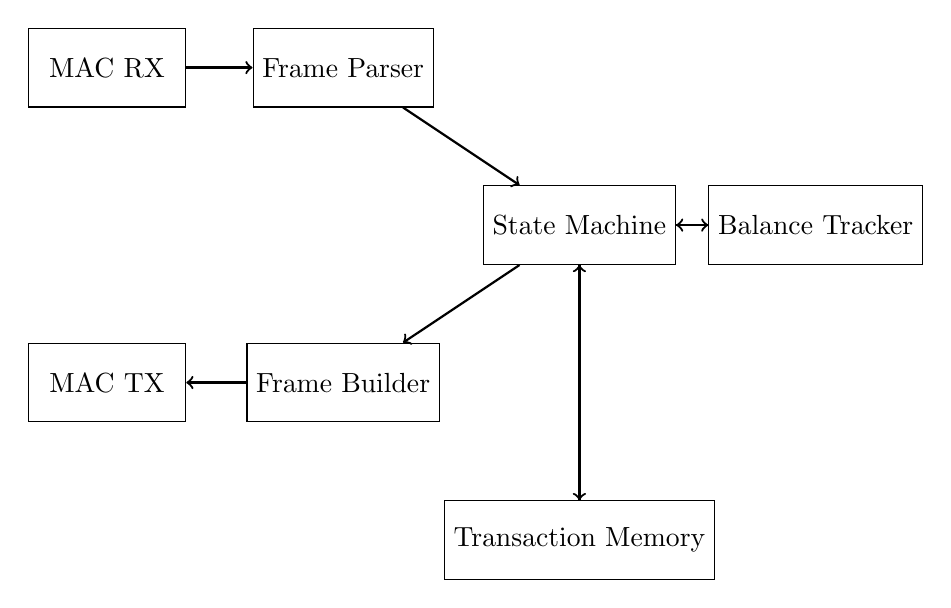
\begin{tikzpicture}[
    module/.style={rectangle, draw, text centered, minimum height=1cm, minimum width=2cm},
    arrow/.style={->, thick}
]
    % Input/Output modules
    \node[module] (mac_rx) at (0,0) {MAC RX};
    \node[module] (mac_tx) at (0,-4) {MAC TX};
    
    % Protocol modules
    \node[module] (frame_parser) at (3,0) {Frame Parser};
    \node[module] (frame_builder) at (3,-4) {Frame Builder};
    
    % Core logic
    \node[module] (state_machine) at (6,-2) {State Machine};
    \node[module] (balance_tracker) at (9,-2) {Balance Tracker};
    
    % Memory
    \node[module] (transaction_memory) at (6,-6) {Transaction Memory};
    
    % Connections
    \draw[arrow] (mac_rx) -- (frame_parser);
    \draw[arrow] (frame_parser) -- (state_machine);
    \draw[arrow] (state_machine) -- (balance_tracker);
    \draw[arrow] (balance_tracker) -- (state_machine);
    \draw[arrow] (state_machine) -- (frame_builder);
    \draw[arrow] (frame_builder) -- (mac_tx);
    \draw[arrow] (state_machine) -- (transaction_memory);
    \draw[arrow] (transaction_memory) -- (state_machine);
\end{tikzpicture}
\caption{FPGA Implementation Architecture}
\end{figure}

\subsection{Registers and Memory Structure}

\begin{table}[h]
\centering
\begin{tabular}{|l|c|l|}
\hline
\textbf{Register} & \textbf{Width (bits)} & \textbf{Description} \\
\hline
STATE\_REG & 3 & Current protocol state \\
BALANCE\_REG & 3 & Current balance indicator \\
TRANS\_ID\_REG & 16 & Current transaction ID \\
TIMEOUT\_COUNTER & 32 & Timeout counter \\
CONTROL\_REG & 8 & Control register \\
STATUS\_REG & 8 & Status register \\
\hline
\end{tabular}
\caption{Register Definitions}
\end{table}

\subsection{Memory Organization}

The Transaction Memory should be implemented as dual-port RAM with the following structure:

\begin{table}[h]
\centering
\begin{tabular}{|l|c|l|}
\hline
\textbf{Field} & \textbf{Width (bits)} & \textbf{Description} \\
\hline
Transaction ID & 16 & Key for the entry \\
Balance State & 3 & Associated balance state \\
Operation & 5 & Associated operation \\
Timestamp & 32 & Timestamp of last activity \\
Data Pointer & 16 & Pointer to data in payload memory \\
Data Length & 16 & Length of associated data \\
\hline
\end{tabular}
\caption{Transaction Memory Structure}
\end{table}

\subsection{Pseudo-Verilog for Core State Machine}

\begin{lstlisting}[language=Verilog]
module cq_state_machine (
    input wire clk,
    input wire reset,
    input wire [2:0] rx_balance,
    input wire [4:0] rx_operation,
    input wire [15:0] rx_transaction_id,
    input wire frame_valid,
    output reg [2:0] tx_balance,
    output reg [4:0] tx_operation,
    output reg [15:0] tx_transaction_id,
    output reg tx_request,
    output reg [2:0] current_state
);

// State definitions
localparam STATE_INIT = 3'b000;
localparam STATE_PLUS_ZERO = 3'b001;
localparam STATE_PLUS_ONE = 3'b010;
localparam STATE_MINUS_ONE = 3'b011;
localparam STATE_MINUS_ZERO = 3'b100;
localparam STATE_PLUS_INF = 3'b101;
localparam STATE_MINUS_INF = 3'b110;

// Operation codes
localparam OP_NOP = 5'b00000;
localparam OP_DATA = 5'b00001;
localparam OP_ACK = 5'b00010;
localparam OP_REQ = 5'b00011;
localparam OP_RSP = 5'b00100;
localparam OP_SYNC = 5'b00101;
localparam OP_SYNC_ACK = 5'b00110;
localparam OP_RESET = 5'b00111;

// Internal registers
reg [31:0] timeout_counter;
reg timeout_occurred;

// State machine logic
always @(posedge clk or posedge reset) begin
    if (reset) begin
        current_state <= STATE_INIT;
        tx_balance <= 3'b000;
        tx_operation <= OP_NOP;
        tx_transaction_id <= 16'h0000;
        tx_request <= 1'b0;
        timeout_counter <= 32'h00000000;
        timeout_occurred <= 1'b0;
    end else begin
        // Default values
        tx_request <= 1'b0;
        
        // Timeout detection
        if (timeout_counter > 0) begin
            timeout_counter <= timeout_counter - 1;
            if (timeout_counter == 1) begin
                timeout_occurred <= 1'b1;
            end
        end
        
        // State transitions based on received frames and timeouts
        case (current_state)
            STATE_INIT: begin
                if (frame_valid && rx_operation == OP_SYNC) begin
                    current_state <= STATE_PLUS_ZERO;
                    tx_balance <= 3'b011; // +0
                    tx_operation <= OP_SYNC_ACK;
                    tx_transaction_id <= rx_transaction_id;
                    tx_request <= 1'b1;
                    timeout_counter <= 32'd100000; // Set appropriate timeout value
                end
            end
            
            STATE_PLUS_ZERO: begin
                if (frame_valid) begin
                    case (rx_operation)
                        OP_DATA: begin
                            current_state <= STATE_PLUS_ONE;
                            tx_balance <= 3'b100; // +1
                            tx_operation <= OP_ACK;
                            tx_transaction_id <= rx_transaction_id;
                            tx_request <= 1'b1;
                        end
                        OP_REQ: begin
                            current_state <= STATE_MINUS_ONE;
                            tx_balance <= 3'b001; // -1
                            tx_operation <= OP_RSP;
                            tx_transaction_id <= rx_transaction_id;
                            tx_request <= 1'b1;
                        end
                        OP_SYNC_ACK: begin
                            current_state <= STATE_MINUS_ZERO;
                            tx_balance <= 3'b010; // -0
                        end
                        // Handle other operations...
                    endcase
                end else if (timeout_occurred) begin
                    // Handle timeout in +0 state
                    timeout_occurred <= 1'b0;
                    tx_operation <= OP_SYNC;
                    tx_transaction_id <= tx_transaction_id + 1;
                    tx_request <= 1'b1;
                    timeout_counter <= 32'd100000;
                end
            end
            
            // Additional states and transitions...
            // STATE_PLUS_ONE, STATE_MINUS_ONE, etc.
            
        endcase
    end
end

endmodule
\end{lstlisting}

\subsection{Test Vectors (Conventional Ethernet)}

The following test vectors can be used to verify the implementation:

\begin{enumerate}
    \item \textbf{Connection Establishment}:
    \begin{itemize}
        \item Node A sends SYNC with balance $+0$
        \item Node B responds with SYNC\_ACK with balance $-0$
        \item Expected outcome: Both nodes establish connection
    \end{itemize}
    
    \item \textbf{Basic Data Transfer}:
    \begin{itemize}
        \item Node A sends DATA with balance $+1$
        \item Node B responds with ACK with balance $+0$
        \item Expected outcome: Data successfully transferred
    \end{itemize}
    
    \item \textbf{Data Request}:
    \begin{itemize}
        \item Node A sends REQ with balance $-1$
        \item Node B responds with RSP with balance $+0$
        \item Expected outcome: Requested data successfully received
    \end{itemize}
    
    \item \textbf{Error Recovery}:
    \begin{itemize}
        \item Node A sends DATA with balance $+1$
        \item Frame is lost (not injected in test)
        \item Timeout occurs at Node A
        \item Node A sends SYNC with balance $+0$
        \item Node B responds with state information
        \item Node A resends missing data
        \item Expected outcome: Error recovered with minimal retransmission
    \end{itemize}
\end{enumerate}

\subsection{Implementation Guidelines (Conventional Ethernet)}

When implementing the CQ protocol in an FPGA, consider the following:

\begin{enumerate}
    \item Use a pipelined architecture to achieve high throughput
    \item Implement the transaction memory as dual-port RAM for simultaneous access
    \item Use a parameterized design to allow configuration of buffer sizes, timeout values, etc.
    \item Include comprehensive error detection and reporting mechanisms
    \item Add debug ports to monitor internal state transitions
    \item Implement the CRC calculation using parallel techniques for high performance
    \item Consider using a dedicated timeout counter for each active transaction
\end{enumerate}

\subsection{Verification Plan (Conventional Ethernet)}

To verify the implementation:

\begin{enumerate}
    \item Use simulation with the provided test vectors to verify basic functionality
    \item Test edge cases such as simultaneous transmissions and maximum-size frames
    \item Measure performance metrics including latency, throughput, and resource utilization
    \item Conduct stress testing with high packet rates and induced errors
    \item Verify interoperability between multiple implementations
\end{enumerate}

\clearpage

\newpage
\section{Atomic Ethernet Frame Format: Æ-Link CQ Interactions}

\begin{table}[h]
\vspace{-10pt}
\begin{tabular}{|l|c|l|}
\hline
\textbf{Field} & \textbf{Size (bits)} & \textbf{Context} \\
\hline
Slice 1 & 8 & OPCODE (Protocol Specifier) \\
Slice 1 & 8 & Liveness  (TIKTIKTIK) \\
Slice 1 & 8 & State  (State Machine Specifier) \\
Slice 1 & 8 & Transition  (State Machine Transition) \\
Slice 1 & 32 & Operand (One-shot CQ Interactions) \\
\hline
Slice 2-8 & 512 & Operand (One-Shot CQ Interactions) \\
\hline
\end{tabular}
\caption{Æ Minimalist CQ Protocol See: Slice Engine: Frame Format Spec.}
\end{table}

\vspace{-10pt}
\section{Slice 1 -- Byte 1Protocol}

\begin{table}[h]
\vspace{-10pt}
\begin{tabular}{|l|c|l|}
\hline
\textbf{Field} & \textbf{Size (bits)} & \textbf{OPCODE} \\
\hline
Slice 1 & 8 & Context (Protocol Specifier) \\
\hline
\end{tabular}
\caption{Protocol Specifier.}
\end{table}

\vspace{-10pt}
\subsection{Slice 1 -- Byte 2 Liveness}

\begin{table}[h]
\vspace{-10pt}
\begin{tabular}{|l|c|l|}
\hline
\textbf{Field} & \textbf{Size (bits)} & \textbf{LIVENESS} \\
\hline
Slice 1 & 8 & IKTYKTIKT (Liveness Specifier)\\
\hline
\end{tabular}
\caption{Liveness Specifier.}
\end{table} 


\end{document}


